\documentclass[uplatex,11pt,a4j,titlepage,oneside,openright,dvipdfmx]{jsbook}
\pagestyle{headings}

%from 000a_header
%\usepackage{bm}
\usepackage{amssymb,amsfonts,amsthm}
\usepackage{amsmath}
%\usepackage{multirow}
\usepackage{url}
\usepackage[dvipdfmx]{graphicx,hyperref}
\usepackage{pxjahyper}
\usepackage{afterpage}
\usepackage{cite}
\usepackage{bm}

\usepackage{color}

\def\vector#1{\mbox{\boldmath $#1$}}

\makeatletter
\renewcommand{\theequation}{\arabic{chapter}.\arabic{section}.\arabic{equation}}
\@addtoreset{equation}{section}
\makeatother

%from jsbook mima version
\setlength{\hoffset}{+00mm}
\setlength{\voffset}{-05mm}
\setlength{\textheight}{36\baselineskip}
\addtolength{\textheight}{\topskip}

\setlength{\oddsidemargin}{-1truein}% いったん左余白を実質上 0pt とする
\addtolength{\oddsidemargin}{1.2truein}% 左余白幅
\setlength{\evensidemargin}{-1truein}% いったん左余白を実質上 0pt とする
\addtolength{\evensidemargin}{1.1truein}% 左余白幅
\textwidth=6.0truein%
\fullwidth\textwidth% ヘッダーの線幅を \textwidth に一致

\usepackage{multicol}
\usepackage{comment}
\usepackage{ulem}

\usepackage{accents}
\usepackage{algpseudocode,algorithm}

%for write C/C++ code
%\usepackage{ascmac}
\usepackage{here}
\usepackage{txfonts}
\usepackage{listings, jlisting}
\usepackage{remreset}

\lstset{language=c,
  basicstyle=\ttfamily\scriptsize,
  commentstyle=\textit,
  classoffset=1,
  keywordstyle=\bfseries,
  frame=tRBl,
  framesep=5pt,
  showstringspaces=false,
  numbers=left,
  stepnumber=1,
  numberstyle=\tiny,
  tabsize=2
}
%lstlistingに章番号を付けない
\makeatletter
\AtBeginDocument{
\@removefromreset{lstlisting}{chapter}
\def\thelstlisting{\arabic{lstlisting}}}
\makeatother

\newcommand{\Tabref}[1]{表~\ref{#1}}
\newcommand{\Equref}[1]{式~(\ref{#1})}
\newcommand{\Figref}[1]{図~\ref{#1}}

\begin{comment}
\hoffset = 0pt
\voffset = 0pt
\topmargin = -72.27pt
\headheight = 25mm
\headsep = 0pt
\oddsidemargin = -15.36542pt
%\textheight = 634pt
\textheight = 247mm
\textwidth = 483.18904pt
%\paperheight = 845pt
\paperheight = 297mm
%\paperwidth = 597pt
\paperwidth = 210mm
\columnsep=28.45274pt

\makeatletter  % --- 「おまじないモード」に入る

\renewcommand{\section}{%
   \@startsection{section}{1}{\z@}%
   {0.5\Cvs \@plus.0\Cdp \@minus.2\Cdp}%  上の空き
   {0.2\Cvs \@plus.1\Cdp \@minus.3\Cdp}%  下の空き
   {\reset@font\large\bfseries}}%         字の大きさ

\makeatother   % --- 「おまじないモード」から抜ける

\makeatletter  % --- 「おまじないモード」に入る

\renewcommand{\subsection}{%
   \@startsection{subsection}{1}{\z@}%
   {0.3\Cvs \@plus.0\Cdp \@minus.2\Cdp}%  上の空き
   {0.1\Cvs \@plus.1\Cdp \@minus.3\Cdp}%  下の空き
   {\reset@font\large\bfseries}}%         字の大きさ

\makeatother   % --- 「おまじないモード」から抜ける
\end{comment}

\begin{document}
\setlength{\baselineskip}{16pt}
\frontmatter

 \thispagestyle{empty}

%\hspace{\fill} {\large 論文番号~5-07~~~~~}
   %\vspace{2cm}
\begin{center}
   \vspace{8.0cm}
    {\LARGE  GENESIS向け\\区間多項式近似短距離力カーネル最適化報告書}\\
   \vspace{3mm}

 \vspace{10.0cm}
 {\Large 12/2018} \\
 \vspace{3.5cm}
 {\LARGE コデザイン推進チーム} \\
 \vspace{1.5cm}
\end{center}
\newpage
\thispagestyle{empty}

\mbox{}\newpage

\thispagestyle{empty}
\begin{center}
 {\LARGE 要約}
 \vspace{2.0cm}
\end{center}
本文書は,分子動力学シミュレーションパッケージソフト「GENESIS」の近距離相互作用計算カーネルのポスト「京」で採用されるプロセッサ「A64FX」に向けた最適化に関する報告書である.
分子動力学シミュレーションソフトでは,その計算時間の大部分を占める粒子間の相互作用計算には,一般にParticle Mesh Ewald(PME)法やFast Multipole法のように,遠くの粒子との相互作用を効率良く計算する方法が用いられることが多い.GENESISで採用されているPME法では粒子間相互作用の成分を距離に応じて急速に減衰する近距離成分と遠距離成分に分けて計算しており,本文書で議論するのは前者の計算速度である.
現在GENESISで採用されている近距離相互作用計算カーネルでは,テーブルから参照した値を線形補間して計算を行っている.この方式は,カーネル内での演算量を劇的に減らせる一方,大きなテーブルへの間接アクセスがボトルネックになっている.
%A64FXは,単精度で16並列のSIMDユニットを持つが,間接アクセスのスループットは通常で1サイクル2語と低いためである.
%これは,キャッシュミスが多く,1サイクルあたりに2語の間接アクセスでの最大スループットが出ていないためである.
%近年作られている他のハードウェアよりは良いとはいえ,メモリバンド幅と演算との比であるB/F値は小さい.
A64FXは,単精度で16並列のSIMDユニットを持つが,間接アクセスのスループットは理想的な場合でも1サイクル2語である.
したがって,同一キャッシュライン上に複数語ある場合を除いては16語をロードするのに8サイクルかかることになる.
さらに,データがL1/L2キャッシュにのっていない場合には大きなペナルティがある(表\ref{tab:A64FX}のメモリレイテンシを参照)ため,参照範囲が広い間接アクセスが大量に発生するような実装は好ましいとは言えない.
したがって,本文書では大きなテーブルへの間接アドレスアクセスを排除するため,SIMDレジスタ数本にのる大きさのテーブルを用いた区間多項式近似を用いた近距離相互作用計算カーネルの最適化を行った結果を報告する.
区間多項式近似カーネルを用いた場合,2018年9月13日時点でのGENESISのNonb15Fカーネルの1ステップあたりの実機での計算時間12.2 msに対して,理研シミュレータにおいて7.87 ms(1.55倍)相当の計算速度を達成した.
精度については,GENESISにおいてテーブル密度を20とした場合と同程度の精度を保っている.
現在,コンパイラのバグや不備,シミュレータと実機の差異によって,性能が低く見積もられていると予測される部分が有り,実機ではさらに1割程度性能が改善する見込みがあると考えている.

 \begin{table*}[b]
  \centering
  \caption{Nonbond\_June1と多項式近似カーネルの比較.ネイバーサーチのマージンを\mbox{1.5 \AA}と想定.}
  \label{tab:comp}
  \begin{tabular}{l||l|l}
   \hline \hline
   カーネル名 & Nonbond\_June1 & 区間多項式近似カーネル \\ \hline
   測定方法 & 実機 & 理研シミュレータ \\
   コアあたり単位時間あたりの相互作用数 & 56.7 M 相互作用/s & 87.94 M 相互作用/s \\
   1チップ48コア換算の1ステップの実行時間 & 12.2 ms & 7.87 ms\\ \hline
   倍率 & 1.00 & 1.55 \\
   \hline \hline
  \end{tabular}
 \end{table*}

\newpage

\setcounter{page}{0}

\setcounter{tocdepth}{2}
%index
\markboth{目次}{}
\setcounter{page}{1}
\tableofcontents

\mainmatter

\chapter{はじめに}
\section{この文書の目的}
この文書では,ポスト京で採用されるA64FXプロセッサ向けに,理研杉田チームで開発されている分子動力学シミュレーションパッケージ「GENESIS」の短距離相互作用の計算カーネルを高速化する手法を検討する.
この章では,カーネルの高速化のために必要なプロセッサやシミュレータに関する事前知識について触れる.次章では,現在のGENESISの短距離力カーネルの概要や実装,ベンチマーク結果を紹介し,\ref{chapter:poly}章では本文書で提案する区間多項式近似手法の概要,最適化手順,ベンチマークの条件,その結果について述べる.

\chapter{測定環境など}
\section{A64FX}
 A64FXはポスト「京」向けに富士通が開発を進めているプロセッサである.A64FXのスペックを表\ref{tab:A64FX}に示す.アーキテクチャにARMv8-Aを採用し,ARM Scalable Vector Extension (SVE)のSIMD命令が使用できる.4つのCore Memory Group(CMG)からなり,各CMGは12個の演算コアと1つのアシスタントコアで構成されている.メモリは4つのHigh Bandwidth Memory 2(HBM2)があり,各CMGに一つずつつながっている.そのため,各CMGからちがうCMGのメモリへアクセスしようとするとアクセス速度が変わる.全体での最大バンド幅は\mbox{1 TB/s}程度である.512 bit幅のSIMD命令が実行でき,理論ピーク性能は倍精度で\mbox{2.7 TFlops},単精度ではその倍である.メモリ階層はL2までの階層キャッシュで,各キャッシュやメモリへのアクセスレイテンシなどは表の通りである.

 以降では,分子動力学シミュレーションコードを最適化するにあたって重要な特徴について述べる.命令はアウトオブオーダー(OoO)実行される.加算や乗算,Multiply and Add (MAD)命令のレイテンシは9と若干大きく,分子動力学シミュレーションなどのレイテンシネックになりやすいアプリケーションではこの長いレイテンシをうまく隠蔽する必要があるが,Simulataneous Multi Thread (SMT)などの演算レイテンシを隠蔽するような機能はハードウェア的にはOoOぐらいしか採用されていない.そのため,演算順序に依存性がある場合,ソフトウェアパイプライニング(SWPL)段数がレイテンシの数を上回らなければ,基本的に理論上到達可能な速度になることはない.演算同士の順序依存性を減らしつつ,レジスタの使用数を抑えながら実装することで,SWPLの段数を増やしてレイテンシが隠蔽される様にする必要がある.レイテンシが9の命令がある場合,Arithmetic Logic Unit(ALU)が2つあるのでSWPLの段数が少なくとも18以上でループ長がループ開始部分のSWPLが効いていない部分が隠蔽される程度長くないと理想的な性能は得られない.これらに関してはロードストアの回数は増えるが,ループ分割を行うなどの対策が有効である.SWPLを有効にするためには,最内側ループにある程度の回転数が必要となるため,分子動力学の様に,ボトルネック部分に2重ループがでてくるアプリケーションでは,可能であれば最内側ループをSIMD化するのは避けるべきであると考えられる.

 \begin{table}
  \caption{A64FXの仕様およびコンパイラのバージョン等.}
  \label{tab:A64FX}
  \begin{tabular}{l|l}
   \hline \hline
   項目 & 説明 \\ \hline
   コア数 / CMG & 12\\
   CMG数 & 4 \\
   ALU / コア & 2 \\
   SIMD幅 & 512 bit \\
   動作周波数 & 1.8 GHz \\
   理論ピーク性能 & 倍精度 2.7 TFlops \\
   SIMDレジスタ数 / コア& 32本 \\
   メモリ(容量,ピークバンド幅) & 4 $\times$ HBM2(32 GB, 256 GB/s)\\
   メモリ階層(レイテンシ) & L1 (5) \\%(SIMD利用時はもう少しかかる模様 by 似鳥さん)\\
   & L2 (42)\\
   & HBM (CMG内 255 / CMG外 420)\\
   コンパイラ & FCCpx (FCC) 1.2.0 20180907 simulating gcc version 4.1.2 \\
   \hline \hline
  \end{tabular}
 \end{table}

\section{理研シミュレータ}
この節では,カーネルの最適化を行う際に使用したA64FXの理研シミュレータと実機との差異,使用したツールについて述べる.
理研シミュレータは,富士通側で使用しているA64FXのシミュレータを理研側では使用できないために理研側で開発されているA64FXシミュレータである.Gem5を利用して作られている.現状,富士通のコンパイラから吐かれたアセンブラを利用して,.axfファイルを作成し,シミュレーションを行う.動作は速いが実際の実行時間を取ることができないatomicというモードと,実行サイクル数から実機での実行時間を予測できるo3というモードがある.以降では,基本的にo3モードを利用した際の話を述べる.
\subsection{実機とシミュレータの差異}
Arm SVE命令は,3オペランドの命令である.そのため,MAD命令を実行する際には,一つのオペランドが入力と出力の両方を担当することになる.そのため,各オペランドの値全てを取っておく必要がある場合,あらかじめ別のレジスタに値を移すことが必要となる場合がある.このときに,movprfxという命令が吐かれる.
A64FXの実機ではこのmovprfxとMAD命令は一つの命令としてデコード・実行されるためmovprfxのレイテンシを気にする必要はない.しかしながら,理研シミュレータでは実装の関係で,movprfxとMAD命令は別々にデコードされ,movprfxも1サイクルのレイテンシがある命令として実行される.そのため,movprfxが頻繁に吐かれるようなコードの場合,MAD命令は実質レイテンシが1サイクル増えることとなるし,movprfxの分もOoO資源などが割かれることになる.
movprfx命令はインアクティブなプレディケートを0で埋める命令の際にも必ず発効される.
SWPLの段数が十分に大きいループでは,すべての命令は実質1サイクルのレイテンシで実行される.理研シミュレータで時間測定を行う場合,本来は隠蔽されるはずのmovprfx命令の割合が大きくループの性能評価に影響を与える可能性があるので注意が必要である.

\subsection{シミュレーション結果の可視化}
本文書で行った最適化では,理研シミュレータで行われたシミュレーションの結果をサイクルレベルでどのようにデコードから実行まで行われているかを可視化するために,フリーウェアのGem5の実行結果可視化ソフトKonata\cite{Konata}を利用した.本文書で述べている演算のレイテンシなどは,シミュレーション結果を可視化した値(つまり,理研シミュレータで設定されている値)を用いている場合が多い.

\chapter{GENESIS}
この章では,GENESIS向け短距離力最適化カーネルを作成するに当たって必要な現状のGENESISの実装やテスト問題に関する情報を示す.

\section{短距離相互作用}
GENESISの短距離相互作用は主に2つの要素に分けられる.一つは,スイッチング関数がかかったLennad-Jones相互作用である.もう一つは,Ewald法を用いて静電相互作用を計算するときの短距離成分である.本報告書で使用したカットオフ距離$r_ c$,スイッチング開始距離$r_s$,Ewald法のパラメータ$\alpha$の設定値を表\ref{tab:parameters}に示す.

\begin{table}
   \centering
  \caption{短距離力計算時のパラメータ.}
  \label{tab:parameters}
  \begin{tabular}{l|l}
   \hline \hline
   $r_c$    & 12 \AA \\
   $r_s$    & 10 \AA \\
   $\alpha$ & 0.34 \\
   \hline \hline
  \end{tabular}
\end{table}

\subsection{スイッチング関数を乗じたLennard-Jones相互作用}
GENESISで採用されているcharmmのLennard-Jonesポテンシャル$U_{\mathrm{LJSW}}(r)$は,一般に用いられる12-6型のLennard-Jonesポテンシャル$U_{\mathrm{LJ}}$とスイッチング関数$S(r)$の積で書けて,
\begin{eqnarray}
 U_{\mathrm{LJSW}}(r) = U_{\mathrm{LJ}}(r) S(r).
\end{eqnarray}
ただし,
\begin{eqnarray}
 U_{\mathrm{LJ}}(r)= 4\epsilon \left\{ \left( \frac{\sigma}{r} \right)^{12} - \left( \frac{\sigma}{r} \right)^{6} \right\},
\end{eqnarray}
\begin{eqnarray}
 S(r) = \left\{
   \begin{array}{ll}
    1 & (r < r_s) \\
    \dfrac{(r_c^2 - r^2)^2(r_c^2 + 2 r^2 - 3 r_s^2)}{(r_c^2 - r_s^2)^3} & (r_s \leq r < r_c) \\
    0 & (r_c \leq r)
   \end{array}
 \right.
\end{eqnarray}
である.
ここで,$\sigma$と$\epsilon$は粒子の直径とポテンシャルの深さを表すパラメータであり,原子種ごとにその値が決まっている.
違う種類の原子同士が相互作用をする場合は,原子$i$と原子$j$のそれぞれの$\sigma$と$\epsilon$を用いて,Lorentz-Berthelot則によって以下の様に決まる.
\begin{eqnarray}
 \sigma &=& \frac{\sigma_i + \sigma_j}{2}, \\
 \epsilon &=& \sqrt{\epsilon_i \epsilon_j}.
\end{eqnarray}

スイッチング関数を乗じたLJ相互作用による力$\bm{F}_{\mathrm{LJSW}}$は,
\begin{eqnarray} \label{eq:LJSW}
 \bm{F}_{\mathrm{LJSW}}(r) = -\dfrac{dU_{\mathrm{LJSW}}}{d\bm{r}} = \left\{
 \begin{array}{ll}
  \bm{F}_{\mathrm{LJ}} & (r < r_s) \\ 
  \bm{F}_{\mathrm{LJ}} S(r) - U_{\mathrm{LJ}}(r)\dfrac{dS(r)}{d\bm{r}}  & (r_s \leq r < r_c) \\
  0 & (r_c \leq r)
 \end{array}
 \right.
\end{eqnarray}
となる.
ただし,$\bm{F}_{\mathrm{LJ}}(r)$と$\frac{dS(r)}{d\bm{r}}$は,
\begin{eqnarray}
 \bm{F}_{\mathrm{LJ}} = -\frac{dU_{\mathrm{LJ}}}{d\bm{r}} = 24\epsilon \left\{ 2\left( \frac{\sigma}{r} \right)^{12} - \left( \frac{\sigma}{r} \right)^{6} \right\}\frac{\bm{r}}{r^2},
\end{eqnarray}
\begin{eqnarray}
 \frac{dS(r)}{d\bm{r}} = \left\{
  \begin{array}{ll}
   0 & (r < r_s) \\
   \dfrac{12(r_c^2-r^2)(r_s^2 - r^2)}{(r_c^2-r_s^2)^3} \bm{r}& (r_s \leq r < r_c) \\
   0 & (r_c \leq r)
  \end{array}
  \right.
\end{eqnarray}
である.

% \begin{eqnarray}
%  U(r) = \frac{A}{12 r^{12}} - \frac{B}{6 r^6} \\
%  \boldmath{F}(r) = \left(\frac{A}{r^{14}} - \frac{B}{r^8} \right) \boldmath{r}
% \end{eqnarray}

% \begin{eqnarray}
%  F_{sw}(r) &=& - \frac{d}{dr}U(r)S(r) = F(r)S(r) - U(r)\frac{dS(r)}{dr} \\
%  &=& \left\{ \left(\frac{A}{r^{13}} - \frac{B}{r^7} \right)\frac{(r_c^2 - r^2)^2(r_c^2 + 2 r^2 - 3 r_s^2)}{(r_c^2 - r_s^2)^3} - \left(\frac{A}{12 r^{12}} - \frac{B}{6 r^6}\right)\frac{12r(r_c^2-r^2)(r_s^2 - r^2)}{(r_c^2-r_s^2)^3} \right\}\frac{r}{r} \\
%  &=& \frac{r_c^2 - r^2}{(r_c^2-r_s^2)^3} \left\{ \left(\frac{A}{r^{13}} - \frac{B}{r^7} \right) (r_c^2 - r^2) (r_c^2 + 2 r^2 - 3 r_s^2) - \left( \frac{A}{12 r^{12}} - \frac{B}{6 r^6} \right) 12r(r_s^2 - r^2) \right\} \frac{r}{r} \\
%  &=& \frac{r_c^2 - r^2}{(r_c^2-r_s^2)^3} \left\{ \left(\frac{A}{r^{14}} - \frac{B}{r^8} \right) (r_c^2 - r^2) (r_c^2 + 2 r^2 - 3 r_s^2) - \left( \frac{A}{r^{12}} - \frac{2B}{r^6} \right) (r_s^2 - r^2) \right\} \boldmath{r} \\
%   &=& \frac{r_c^2 - r^2}{(r_c^2-r_s^2)^3} \left\{ \frac{A}{r^{14}}(r_c^2 - r^2) (r_c^2 + 2 r^2 - 3 r_s^2) - \left( \frac{A}{r^{12}} - \frac{2B}{r^6} \right) (r_s^2 - r^2) \right\} \boldmath{r}
% \end{eqnarray}

\subsection{Ewald法を用いた静電相互作用の短距離成分}
粒子$i$と$j$の電荷をそれぞれ$Q$,$q$としたとき,粒子間の静電ポテンシャルは以下の様に表される.
\begin{eqnarray}
 U_{\mathrm{CLMB}}(r) = \frac{Qq}{4\pi\epsilon_0r}.
\end{eqnarray}
ここで,$\epsilon_0$は真空の誘電率である.
静電ポテンシャルは,LJポテンシャルと違い$r$に対する減衰が遅い関数であり,周期境界条件下ではシミュレーションセルの周りに存在するイメージセルの寄与を考慮する必要があるが,本報告書では長距離力を考慮せず短距離力についてのみ議論をするため,粒子$i$と$j$の間の距離は,シミュレーションセル及びイメージセルの中の$j$粒子の中で$i$粒子と最も近いものとの距離とする.

周期境界条件で静電相互作用を高速に計算できるEwald法では,この相互作用を0への収束の早い近距離成分と収束の遅い遠距離成分と自己相関項に分解される.
\begin{eqnarray}
 U_{\mathrm{CLMB}}(r) = U_{\mathrm{short}}(r) + U_{\mathrm{long}}(r) = \mathrm{erfc}(\alpha r) U_{\mathrm{CLMB}}(r) + \mathrm{erf}(\alpha r) U_{\mathrm{CLMB}}(r).
\end{eqnarray}
ここで,$\alpha$はEwald法におけるパラメータであり,計算の精度と速度を考慮して決定される.実際のプログラムにおいては,$\alpha$は実行時にユーザが決定する.また,$\mathrm{erf}(\alpha r)$と$\mathrm{erfc}(\alpha r)$は誤差関数と補誤差関数と呼ばれる.
\begin{eqnarray}
 \mathrm{erfc}(x) = 1 - \mathrm{erf}(x) = \int_{0}^{x}e^{-t^2}dt.
\end{eqnarray}
したがって,近距離成分のポテンシャル$U_{\mathrm{short}}$と力$\bm{F}_{\mathrm{short}}$は,補誤差関数と指数関数を用いて以下のように表される.
\begin{eqnarray} \label{eq:pot_clmb}
 U_{\mathrm{short}}(r) = \frac{Qq}{4\pi\epsilon_0} \frac{\mathrm{erfc}(\alpha r)}{r},
\end{eqnarray}
\begin{eqnarray} \label{eq:Coulomb}
 \bm{F}_{\mathrm{short}}(r) = -\frac{dU_{\mathrm{short}}}{d\bm{r}} = \frac{Qq}{4\pi\epsilon_0} \left\{ \frac{\mathrm{erfc}(\alpha r)}{r^2} + \frac{2\alpha}{\sqrt{\pi}}\frac{\exp(-\alpha^2r^2)}{r}\right\}\frac{\bm{r}}{r}.
\end{eqnarray}


 \section{短距離力カーネルの実装}
 現状のGENESISでは,事前に上記2つの相互作用(LJ相互作用を$1/r$の引力項と斥力項に分けるので実際には3つの項)を計算して2粒子間の距離$r$の関数としてテーブル化する.
 カーネルの最内ループでは,計算された$r$の近傍点から線形補間して計算を行っている.
 テーブルの大きさはテーブルの密度の設定にもよるが数千点から数万点程度とっており,LJ相互作用用に2つ,静電相互作用用に1つのテーブルを保持している.
 これらのテーブルは,L1キャッシュに載りきる大きさではなく,カーネルの実行時間が頻繁に起こるテーブルのメモリもしくはキャッシュへのアクセス速度で律速すると予想される.
 実際,Kernel\_June1では,演算待ちよりもメモリアクセス待ちの時間が大半を占めている(図\ref{fig:genesis_profile}).

 \begin{figure}
 \centering
 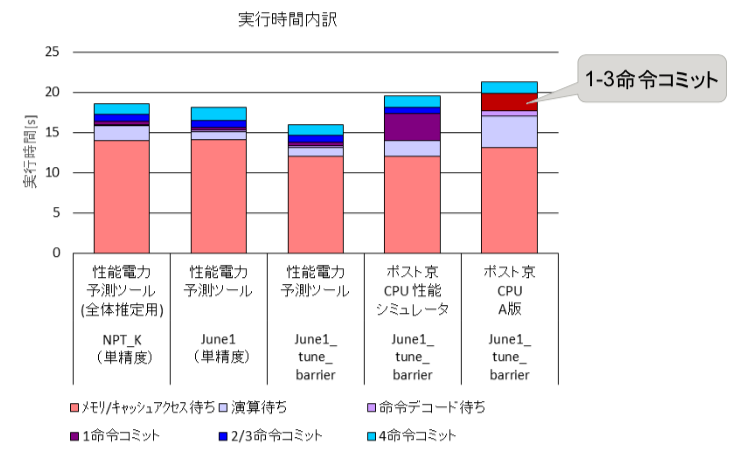
\includegraphics[bb=0 0 734 457, width=12.0cm]{figure/genesis_profile.png}
 \caption[]{カーネルWGで提示されたGENESISのNonb15Fカーネルの予測ツール,シミュレータ,実機での実行時間内訳.ピンク色のメモリ/キャッシュアクセス待ちが演算時間の大半を占める.実機では演算待ちも少し多くなっている.}
 \label{fig:genesis_profile}
 \end{figure}

 \section{Kernel\_June1のシミュレータおよび実機での測定状況} \label{sec:current_situation}
 %測定環境について述べる
 GENESISのベンチマークには,Apoa1と呼ばれるテスト系が用いられている.
 この系は,シミュレーションセルのサイズが$108.861198$ \AA $\times 108.861198$ \AA $\times 77.758003$ \AA で,そのなかに\mbox{92227個}の原子が入っている.
 表\ref{tab:parameters}に示した通りカットオフ半径が\mbox{12 \AA}で系の密度が一様だと仮定すると,カットオフ半径の球体内には約724個の原子が存在することになる.よって,1つの粒子は,平均して中心の粒子を除く\mbox{723個}の粒子と相互作用することになると考えられる.
 Apoa1を入力にGENESIS v1.3.0を実際に実行したときには,1ステップあたりの作用反作用を考慮した相互作用数の数は,\mbox{33.2 M相互作用}であった.上記の一様な密度の仮定でも,\mbox{$92227 \times 723 / 2 = 33.4$ M相互作用}であり,概ね一致している.実行時の相互作用数が若干少ないのは,一様密度の仮定では分子内の隣接原子を相互作用対象から取り除いていないためであると考えている.
 9月13日時点のGENESISの実機での計測では,Nonbond\_June1カーネルでは1ステップあたり\mbox{12.2 ms}かかっている.この実行時間はシミュレータ比1.08倍である.実機測定は48コア実行想定の1ステップあたりの時間であるので,1コアあたりの計算性能は,\mbox{33.2 M相互作用 / (12.2 ms $\times$ 48 core) = 56.7 M相互作用/s}となる.本報告書では,GENESISの短距離力カーネルの現状の性能値を,1コアあたり\mbox{56.7 M相互作用/s}(作用反作用を考慮),もしくはApoa1入力時の1チップ換算の1ステップの実行時間が\mbox{12.2 ms/step}として,最適化カーネルとの比較を行う.

 \chapter{区間多項式近似カーネル} \label{chapter:poly}
\section{MDシミュレーションパッケージでの短距離力カーネルの実装}
GENESISの実装のようなテーブルを利用した相互作用の計算方法は,さまざまなポテンシャル形に対応しやすいなどのメリットもあり様々なパッケージでも用いられていることはあるが,静電相互作用に限って言えばよく用いられている分子動力学シミュレーションパッケージでは素直に,もしくは$\mbox{erfc}(x)$や$\exp(x)$の項を近似するなど工夫して近距離相互作用をSIMD化した実装が一般的である.
512-bit SIMDのカーネルを持つMDシミュレーションパッケージで最も計算速度が速いものの一つと思われるGROMACSを例にとっても,ミニマックス多項式近似を用いて,$\alpha^2 r^2$を引数に
\begin{eqnarray} \label{eq:gromacs_approx}
f(\alpha^2 r^2) = \frac{2}{\sqrt{\pi}} \frac{\exp(-\alpha^2 r^2)}{\alpha^2 r^2} - \frac{\mathrm{erf}(\alpha r)}{\alpha^3 r^3}
\end{eqnarray}
を高速に求める関数を実装している.
しかしながら,この近似は次数が多く途中で逆数の計算も一度入るため,依然として計算量は少なくない.
さらに計算量を減らすための手法として,本報告書ではさらに効率的な近似方法として区間多項式近似を行う手法を提案する.

\section{512 bit SIMDに適応した多項式近似の方法}
ARM SVE命令には512 bitのレジスタから,インデックスを用いてレジスタの要素を並び替えるtbl命令が存在する.
本手法ではそのtbl命令に着目し,計算量の多い式を区間多項式で近似し,
その係数をレジスタ上に保持しながら計算を行うことによって高速化を図る.

一定の距離で十分に小さくなる短距離力では,一般にカットオフ距離で計算を打ち切る手法を用いることが多い.
そのため,その相互作用を計算する領域を$m$個に分割し,それぞれの区間で$n$次多項式で近似することを考える.
ここで,単精度で計算することを考えると,$m=16$のときには$n+1$本の512 bitレジスタに区間多項式の係数全てをレジスタに載せることができる.

ここで問題となるのが,関数をどう多項式近似するかと計算領域の分割法である.
まず,前者について述べる.
Ewald法の静電相互作用短距離成分は,計算領域内での変化が10桁以上の広範な桁にわたる関数である.
特に,粒子間の距離$r$が小さいときには大きく変化する.
そのため,区間によっては近似の次数$n$を上げなくては十分な精度が得られない.
もう一度静電相互作用の短距離成分の式を示す.
\begin{eqnarray}
 \bm{F}_{ij}(r) = \frac{Qq}{4\pi\epsilon_0} \left\{ \frac{\mathrm{erfc}(\alpha r)}{r^2} + \frac{2\alpha}{\sqrt{\pi}}\frac{\exp(-\alpha^2r^2)}{r}\right\}\frac{\bm{r}}{r}
\end{eqnarray}
これを$R=\alpha r$の関数だと考えると,
\begin{eqnarray}
 \bm{F}_{ij}(R) = \frac{Qq \alpha^3}{4\pi\epsilon_0} \left\{ \frac{\mathrm{erfc}(R)}{R^2} + \frac{2}{\sqrt{\pi}}\frac{\exp(-R^2)}{R}\right\}\frac{\bm{r}}{R}
\end{eqnarray}
となる.このようにすることで,係数を除けば,プログラム実行時に決定する$\alpha$に依存しない関数となる.
つまり,
\begin{eqnarray}
 f(R) = \frac{\mathrm{erfc}(R)}{R^3} + \frac{2}{\sqrt{\pi}}\frac{\exp(-R^2)}{R^2}
\end{eqnarray}
を考えれば良い.
この関数は,$R=0$付近で発散し,$R$が小さい時に大きく値が変化する関数である.
実際のプログラムの中では,LJ相互作用はナイーブに計算することを考えると,力の計算を行う際に必ず$1/r$(もしくは$1/r^2$)を計算している.そのため,この関数に$R$の累乗をかけた関数から目的の値を得ることは乗算数回で得ることができる.
さらに,目的の関数自体の$N$乗根を近似多項式から得て,その値を$N$乗すれば,演算回数を大きく増やさずに近似する関数型を変えることができる.
図\ref{fig:func}に検討した様々な関数形を示す.
ここで,$f(x)$から$f(x)*x^4$(紫,緑,水色,橙色,黄色)までを見ると,$f(x)*x^3$(橙色)が最も$r$が小さい時に値が変動しないことがわかる.さらに,$\sqrt{f(x)*x^3}$は$f(x)*x^3$に比べて$r$が大きい時にも大きく値が変化していないことがわかる.
本手法では,$R$が小さい時と大きい時共に変化が少なく,緩やかに減少していく$\sqrt{f(R)R^3}$を近似対象とした.この関数を使うと,$F_{ij}(R)$の係数部分に含まれる$\alpha^3$と$R^3$に含まれる$\alpha^3$が打ち消しあい,近似値を2乗した値に$1/r^3$を乗じると$f(x)$を得ることができる.実際の計算では,$\alpha r$よりも$(\alpha r)^2$の方が演算数が少なく求まるため,$(\alpha r)^2$から近似を行う.

\begin{figure}
 \centering
 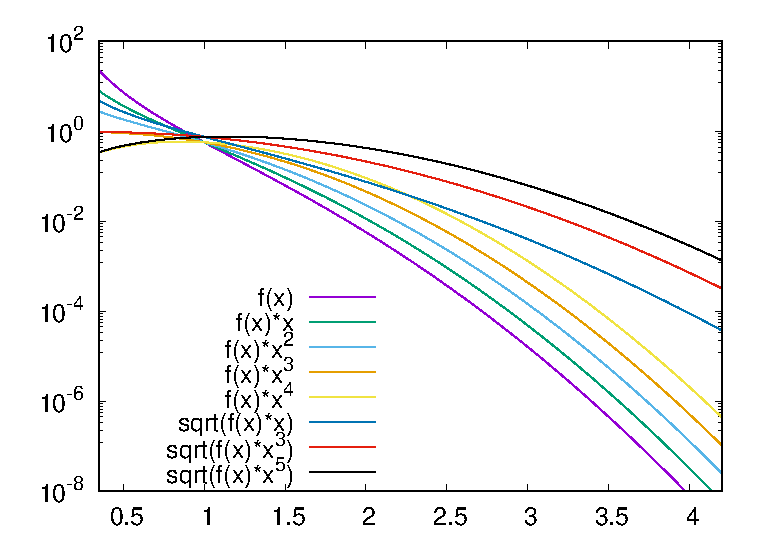
\includegraphics[width=12.0cm]{figure/func.eps}
 \caption[]{静電相互作用の短距離成分の関数形の検討.}
 \label{fig:func}
\end{figure}

次に,近似する領域の分割方法について述べる.
近似する区間の分割方法が決まると,ある程度の精度を保つために近似の次数が決まる.

本カーネルでは,A64FXのSIMD幅に合わせて16点の区間に区切ることを考える.
静電相互作用の短距離成分は,$r$が大きくなるにつれて値が小さくなるため,2粒子間の距離が近いほど近似の精度を上げる必要がある.
しかしながら,複雑な分割区間の設定は計算負荷上好ましくない.
本手法では,$(\alpha r)^2$の$i$番目の区間を$[2^{i-7}, 2^{i-6})$として多項式近似を行った(近似可能な範囲を$0.0078125 \leq (\alpha r)^2 < 512$,および$0.08838834764/\alpha \leq r < 22.627416998/\alpha$とするため).
このような区間の設定を行うと,最初の区間の視点を決めれば$R$の指数部の該当部分\mbox{$\log_2 m$ bit}を取り出すことで,どの区間の近似式を計算するのか$i$を決定できる.
また,倍精度で計算した静電相互作用の短距離成分との絶対誤差がGENESISの線形補間を用いた計算とほぼ同程度もしくはそれ以下にになるように近似の次数$n$を5とした.

$n=5$,$m=16$の時の$\sqrt{f(R)R^3}$を近似して求めた静電相互作用の短距離成分とKernel\_June1で採用されている線形補間から求めた値(GENESISでのパラメータ,table densityは20)を比較する(図\ref{fig:key4_0_5th}).
図\ref{fig:key4_0_5th}は倍精度でナイーブに静電相互作用を計算した場合との誤差を示しており,上段が絶対誤差(差の絶対値),下段が相対誤差(絶対誤差を静電相互作用の値で割ったもの)である.区分多項式(e4bit,m0bit,5th)は概ね全ての領域で線形補完(genesis)を下回っており精度に問題がないことがわかる.$r$の小さい区間で精度が落ちている部分もあるが,相対誤差としては$10^{-7}$程度であり,単精度の範囲では問題無いと考える.また,原子同士が\mbox{$1$ \AA}程度まで近づくことはまれである.
\begin{figure}
 \centering
 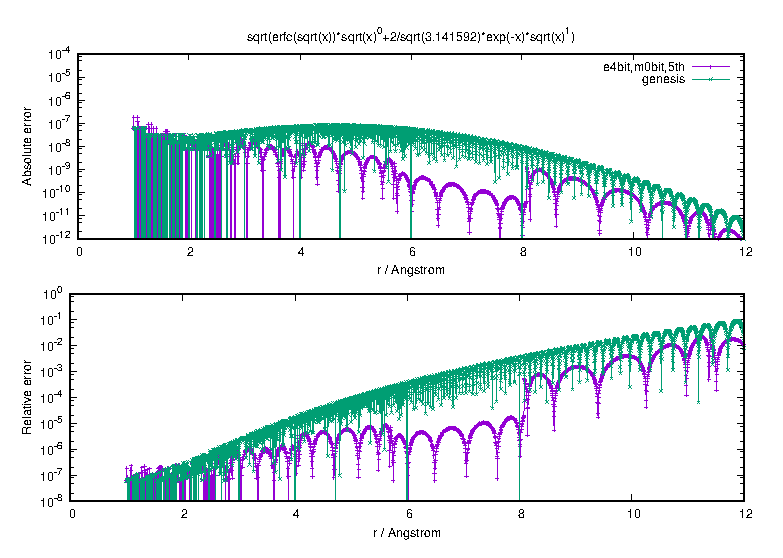
\includegraphics[width=12.0cm]{figure/key4_0_5th.eps}
 \caption[]{区分多項式近似と線形補間の精度比較.比較対象は倍精度でナイーブにF(R)を計算した値.}
 \label{fig:key4_0_5th}
\end{figure}

区間多項式近似の最適な係数を求める際にはSollya\cite{Sollya}というプログラムを用いた.
本手法で用いた係数を出力するためのスクリプトは付録のAlgorithm\ref{algo:sollya}に示す.
Sollyaを用いて求めた$6\times16$個($n$次近似多項式では$n+1$個の定数が必要となる)の定数をSIMDレジスタに載せて演算を行うことを考える.
計算手順はAlgorithm\ref{algo:PPA}の様になる.Sollyaから求めたテーブルは$t$に入っている.実際には6本のSIMDレジスタにそれぞれ$t[0]$から$t[5]$までが載っている.
まず,$x=(\alpha r)^2$を計算する.次に,$x$を23ビット右シフトしてから下位4ビットを取得することで,$x$が$m$個の区間の何番目に含まれているかを計算する($i$).
この際,浮動小数点数では,指数部に下駄履き表現を使っているので,定数を足している.
$i$番目の区間の始まり$x_m$は$i$から求めることができる(ここでは$x_m = 2^{i-7}$)ので$dh = x - x_m$を求めることができる.
あとは,$dh$とテーブル$t$から$n$次多項式の計算を行うだけである.
$n$次多項式の$k$番目の係数$t[k][i]$は,ARM SVEやIntel AVX-512などでは,それぞれtblやpermutexvarなどのSIMD命令を使えば,
SIMDの各要素の$x$から求めたそれぞれの$i$をインデックスとして,並べ替えた値を得ることができるため,SIMD化は容易である.
静電相互作用の近距離成分の演算量を減らせる一方,テーブルを$N+1$本のレジスタで保持しなくてはならないため,A64FXではSWPLの段数を上げることが難しいことが欠点である.

\begin{algorithm}
 \caption{区間多項式近似の計算方法} \label{algo:PPA} % piecewise polynominal approximation
 \begin{algorithmic}
  \Require
  \State $t$[6][16] : $16 \times 6$のテーブル
  \State (to\_float)や(to\_int)は32bit整数や32bit浮動小数の各ビット変化させずにfloatやintに変換するキャスト
  \Function{PollynomialApproximation}{$r$, $\alpha$}
  \State 1 $x  \leftarrow (\alpha r)^2$
  \State 2 $i  \leftarrow (($(to\_int)$R+$0x44000000$) >> 23)$ \& 0x0f
  \State 3 $dh \leftarrow x - $(to\_float)$(i<<23 - \mathrm{0x44000000})$
  \State 4 \Return $t[0][i] + dh*(t[1][i]+ dh*(t[2][i] + dh*(t[3][i] + dh*(t[4][i] + dh*t[5][i]))))$
  \EndFunction
 \end{algorithmic}
\end{algorithm}

\section{最適化カーネルでの前提条件}
% 区間多項式近似によるカーネルでは,SIMD化の関係でKernel\_June1で使用されているようなある粒子と相互作用する粒子のインデックスを持っておくネイバーリスト方式の計算手法を取るためには,粒子データにランダムアクセスをしてSIMD幅に並べる必要がありボトルネックになる可能性がある.
% 本手法では,ネイバーリストを持たず,近隣セル内の粒子全てとの相互作用計算を行うKernel\_DecJulyの方式を採用することにした.
A64FX上で理想的な速度を達成するには,SWPLの効果を活用するために最内側カーネルの回転数がある程度大きいことが求められる.
そのため,本カーネルでは相互作用計算の外側ループ(相互作用を受ける粒子のループ,$i$ループ)をSIMD化を行うこととした.
内側ループ(相互作用を与える粒子のループ,$j$のループ)では,メモリ上に連続なSIMD幅(16個)分の粒子に共通のネイバーリストを作成し,$j$粒子の情報をSIMDレジスタ内で放送して,相互作用の計算を行っている.
理想的な性能に近づけるには最内側ループのSWPLの段数を上げる必要があるため,最内側ループはそれぞれ,$r^2$計算ループ,$1/r$計算ループ,LJ相互作用計算ループ,スイッチング関数計算ループ,区間多項式近似の区間計算ループ,多項式計算ループ,静電相互作用計算ループ,アキュムレート及び反作用計算ループの8つのループに分割を行った.

\subsection{入力データ}
シミュレータ実行時の入力データは以下の様に作成した.
\begin{enumerate}
 \item GENESIS(v1.3.0)を実際に実行し,Apoa1の力の計算を実行.
 \item その際に生成された実際のセル情報および粒子データとセルーセル間のペアリストをファイルに出力.
 \item 必要なサイズに切り出して(セルーセルペアリスト情報から相互作用計算を行うセルとその周りのセルのみを取り出す)入力ファイルを生成.
\end{enumerate}
実際の入力データとしては,相互作用を受けるセルの数を2つとし,2つのセルおよび相互作用を及ぼす周辺のセルを取り出した.
1つのセルに対しては,$5^3 = 125$のセル(自セル含む)が相互作用を及ぼす.

\subsection{入力データの性質}
セル内に含まれる粒子数の累積分布関数を図\ref{fig:cell_size_cumulative_func}に示す.
セル内の粒子数は$0 < N < 80$の範囲に存在し,そのほとんどが50前後に分布していることがわかる.
そのため,極端に小さいセルを大量に含む部分でカーネルの性能を測定しない限りは妥当な見積であると考える.
\begin{figure}
 \centering
 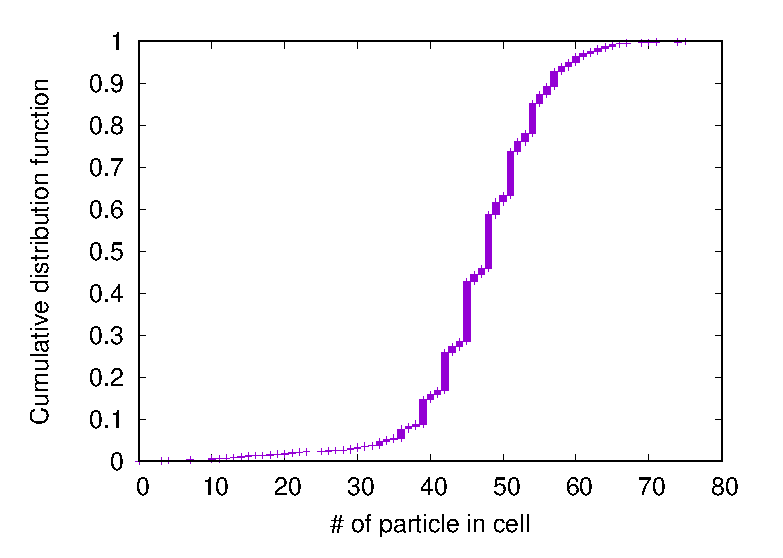
\includegraphics[width=12.0cm]{figure/cell_size.eps}
 \caption[セル内に含まれる粒子数の累積分布関数]{セル内に含まれる粒子数の累積分布関数.}
 \label{fig:cell_size_cumulative_func}
\end{figure}

\subsection{粒子データの並べ方} \label{sec:data_align}
テストコードでは,長めの1次元配列を確保し,セル番号の小さい方から順番に,入力データから得た粒子のデータを連続に詰めている.
その際,粒子データは128 bitアライメントされており,座標の3つの浮動小数点数($x,y,z$)と下位24 bitがその粒子が所属する分子のIDを,上位8 bitが原子の種類を表す32bit符号なし整数($w$)が入っている.
これは,相互作用計算の時にi粒子のデータをSVEのストラクチャーロード命令(ST4)を用いて$x$,$y$,$z$,$w$それぞれの方向に並べ替えるためである.
同様に,力の配列も$x$,$y$,$z$,$w$の4要素ベクトルが並んでいる形になっている.
GENESIS本体の配列構造とは異なるが,カーネル計算時の座標配列は作業用の一時的な配列であるため,比較的簡単に対応可能だと考えている.

また,座標データとは別に,各粒子の電荷$q$は連続な一次元配列上に,LJパラメータ$\sigma$,$\epsilon$は,$w$の上位4 bitの情報からアクセスできる2次元のテーブルに納められている.

\subsection{排除リストの取り扱い}
GENESISでは,相互作用リストを作成する際に分子内の近距離原子に対して排除リストを反映させている.
SIMD環境で排除リストを考慮しながら計算を行うことは実装上難しいため,本カーネルでは同一分子内の原子同士では相互作用の計算はマスクして行わないこととした.
そのため,分子内の相互作用に関しては別途計算を行うことが必要となるので注意されたい.本文書では分子内相互作用の計算速度には触れない.
同一分子かどうかの判定には$w$の下位24 bitを用いている.

\section{シミュレータを用いた最適化}
%演算におけるMAD命令の比率
% あるループを実行する際のシリアルに計算を実行する際の総レイテンシを$L$,ループ内の浮動小数点演算数を$n$,動作周波数を$\nu$,ALUの数を$a$,SIMD幅を$w$,SWPLの段数を$s$として,そのループの理想的な演算性能$P$をラフに見積もる.
% レイテンシネックでALUが十分に使い切れていないと仮定する.総レイテンシが$L$でSWPLの段数が$s$のとき,各ALUに演算が詰まっていくことを考えると,1ループは$La/s$サイクルで回ることになる.1ループの演算量は$nw$なので,
% \begin{eqnarray}
%  P = \frac{nws\nu}{La}
% \end{eqnarray}
% となる(ただし,$s$が大きくなりすぎても,理論ピーク演算性能は越えないものとする).
ここでは例として2粒子間の距離を計算するループについて考えてみる(Algorithm \ref{algo:r2}).
%SWPLが十分に効いていれば十分にレイテンシが隠蔽されるので,
SWPLが十分に効いていれば,二つのALUはそれぞれ自分が担当する別個のループを処理してるともみなせるので,
ここでは一つのALUに演算を詰めていくことを考える.
$dx$と$dy$,$dz$の演算はそれぞれに依存関係がないため,直前の命令が終わった後,すぐに演算を実行することができる.
$r^2$の最初のMAD命令は$dx$と$dy$の演算が終わるまで待つ必要がある.
同様にそれ以降のMAD命令は全て依存関係のある演算なので,直前の演算が終わるまで実行を待つ必要がある.
また,MAD命令の前にはmovprfx命令が発効されている.
$j$粒子のロード命令のレイテンシは6,ストアは命令の発行のみを行えば良いのでレイテンシは1とする.
$j$粒子のロード命令の後には,SIMDレジスタへブロードキャストを行うdup命令が発行される.この命令のレイテンシは4である.
浮動小数演算命令のレイテンシは9なので,依存関係を考慮した場合のSWPLが効いていない場合の1回転あたりのサイクル数は49である.
SWPLの段数が十分に大きいとき,全ての命令のレイテンシは隠蔽されるため,このループは発効される命令の数である16サイクルで実行でき,そのときの性能は\mbox{16 SIMD $\times$ 2 ALU $\times$ 1.8 GHz $\times$ 9 flops / 16 cycle = 32.4 GFlops}となる.
%ロード・ストアのためのアドレス計算も入れると20サイクルになり,\mbox{25.92 GFlops}となる.
%A64FXの動作周波数は1.8 GHz,ALUは2つ,単精度でのSIMD幅は16なので,このループのコアあたりの理想的な性能は\mbox{3.50$s$ GFlops}となる.
%ただし,SWPLの段数が6段を越えて大きくなると,$dx$,$dy$,$dz$の依存関係を考慮しないときの総レイテンシ\mbox{$L=54$サイクル}に近づけて計算する必要が出てくる(\mbox{4.8$s$ GFlops}).
%6命令に占めるMAD命令の数が3つなので,理論ピーク演算性能は3/4になるのでコアあたりでは\mbox{84.4 GFlops}である.そのため,理想的には25段程度のSWPLが必要になることがわかる.
このループの実際のSWPL段数とシミュレータの実行結果から得られた演算性能は,それぞれは9段と\mbox{21.29 GFlops}であった.SWPLの段数は命令のレイテンシを隠蔽するのには十分であるが,実際にはロード・ストア時のアドレス計算などがあるため,このような演算数の少ない短いループの場合,この程度の差は許容範囲であると考える.9段のSWPLのループでは,$r^2$計算に関係ある命令が151,それ以外の命令が82命令あった.\mbox{32.4 $\times$ 151 / (151 + 82) = 21.0 GFlops}となり,概ね測定結果と一致する.
分割した他ループについても同様の検討を行い,そのループでボトルネックを考慮した上では理想的に近い性能が出ていることを確認している.SWPL非適用時に各ループの浮動小数演算が理想的に実行できた場合に各演算がどのような依存関係で実行され,何サイクルかかるのかは別資料を参照されたい.

%表\ref{tab:perf_anal}に分割されたループの演算数,サイクル数,SWPL段数,シミュレータから得られた実際のサイクル数と実効性能を示す.

\begin{algorithm}
 \caption{粒子間距離の計算のループ} \label{algo:r2}
  \begin{algorithmic}
   \Require
   \State $x_i$, $y_i$, $z_i$ : $i$粒子の$x$, $y$, $z$座標
   \State $x_j$, $y_j$, $z_j$ : $j$粒子の$x$, $y$, $z$座標
%   \State $\epsilon$ : $r^2$がゼロにならないための十分に小さい値
   \Function{CalcSquareDistance}{$x_i$, $y_i$, $z_i$, $x_j$, $y_j$, $z_j$}
   \State load $x_j$, $y_j$, $z_j$
   \State broadcast $x_j$, $y_j$, $z_j$ to SIMD register
   \State $dx \leftarrow x_i - x_j$
   \State $dy \leftarrow y_i - y_j$
   \State $dz \leftarrow z_i - z_j$
%   \State copy $dx$ to $dx'$
   \State $r^2 \leftarrow dx*dx$
%   \State copy $dy$ to $dy'$
   \State $r^2 \leftarrow r^2 + dy*dy$
%   \State copy $dz$ to $dz'$
   \State $r^2 \leftarrow r^2 + dz*dz$
   \State store $dx$, $dy$, $dz$, $r^2$
   \EndFunction
  \end{algorithmic}
\end{algorithm}

\section{各種測定}
本節では,区間多項式近似を用いたカーネルについて,2つのケースの性能について議論する.
以下では,理研シミュレータを用いて,1コアでの性能を測定しているものとする.
シミュレータを用いる都合上,計算時間の都合でApoa1の全ての粒子の相互作用を計算することは難しいため,$i$粒子80個分についてのみ相互作用を計算する.表\ref{tab:sim_cond}に計算条件を示す.
コンパイルオプションには「-O3 -Kfast -Kocl -Kswp\_strong -Knosch\_pre\_ra,nosch\_post\_ra」を用いた.
 \begin{table}
  \caption{パフォーマンス測定における$i$粒子の数と各SIMDループにおける$j$ループの長さ.}
  \label{tab:sim_cond}
  \centering
  \begin{tabular}{l||l l}
   \hline \hline
   $i$粒子数 & & 80 \\ \hline
   $j$粒子数 & ループ0 & 1294 \\
            & ループ1 & 1244 \\
            & ループ2 & 1641 \\
            & ループ3 & 1577 \\
            & ループ4 & 1388 \\ \hline
            & 計    & 7144 \\ \hline \hline 
  \end{tabular}
 \end{table}
 
%\subsection{精度の検証} 
%本検証では,実際に倍精度で式\ref{eq:LJSW}と\ref{eq:Coulomb}から計算された力を基準に,単精度でGENESISのテーブルを使って計算された力と本カーネルから求まった力の比較を行った.
 
\subsection{\mbox{$N^2$}計算の場合のパフォーマンス}
まず,ARM SVEを用いて実装したナイーブなLJ相互作用及び区間多項式近似を用いた静電相互作用計算カーネルがA64FXにおいて理想的な場合にどの程度の性能を達成できているかを確認するために,カットオフや分子内相互作用計算を排除しない場合の計算性能について見ていく.
ここでは,静電相互作用やLJ相互作用の係数は定数とみなす.また,本来はネイバーリストを介して不連続にアクセスされる$j$粒子は,メモリ上に連続に並んでいるものとする.また,ここでは周期境界条件や作用反作用は考慮しない.
実際にはカットオフされたり,排除されたりする粒子についても相互作用計算を行うので,相互作用の値は実際のものとは異なっている場合があるが,ここでは純粋にカーネルの速度を測ることを目的とする.

1ループ16粒子に対して,合計で7144個の$j$粒子が存在するため,相互作用数は$16 \times 7144 = 114304$である.
このときの計算時間は\mbox{0.276 ms}であったので,実効性能は\mbox{414.14 M相互作用/s}である.
本カーネルの総浮動小数点演算命令の約半分がMAD命令のため,コアあたりの到達可能なピーク性能は$115.2 * 3 / 4 = 86.4$ GFlopsである.
1相互作用あたりの演算数を73とすると,$N^2$計算カーネルの性能は,\mbox{30.23 GFlops}となり,ピーク性能の約\mbox{35 \%}の性能がでている.
%ただし,計測時間の問題で,相互作用を受ける粒子($i$粒子)は256に限定している.そのため,実際の相互作用の数$256*(512-1) = 130816$である.
%シミュレータ実行によるこのカーネルの計算時間は\mbox{0.255 ms}なので,1秒あたりに計算できる相互作用数は\mbox{513 M相互作用}(作用反作用を考慮しない)となる.
%本カーネルの総浮動小数点演算命令の約半分がMAD命令のため,コアあたりの理論ピーク性能は約$115.2 * 3 / 4 = 86.4$ GFlopsである.
%1相互作用あたりの演算数を73とすると,$N^2$計算カーネルの性能は,37.45 GFlopsとなり,理論ピークの約43\%の性能がでている.

% ----------------------- %
% # of i-cell: 2
% # of i atoms is 80 = (16*5)
% r_c = 12.000000, r_s = 10.000000, r_m = 0.000000, b = 0.340000
% nlist[0] = 1294 (= 0 + 1294)
% nlist[1] = 1244 (= 0 + 1244)
% nlist[2] = 1641 (= 0 + 1641)
% nlist[3] = 1577 (= 0 + 1577)
% nlist[4] = 1388 (= 0 + 1388)
% # of j particles is 7144
% LIST:	   0.000513864 sec
% PRE:	   0.000001155 sec ( 0.42 %)
% POST:	   0.000000784 sec ( 0.29 %)
% r2:	   0.000048107 sec (17.58 %)
% rinv:	   0.000018730 sec ( 6.85 %)
% lj:	   0.000028285 sec (10.34 %)
% switch:	   0.000047904 sec (17.51 %)
% clmb0:	   0.000026979 sec ( 9.86 %)
% clmb1:	   0.000039852 sec (14.57 %)
% clmb2:	   0.000017365 sec ( 6.35 %)
% nwtn3:	   0.000042643 sec (15.59 %)
% other:	   0.000003708 sec ( 1.36 %)
% total time:          0.000275512 sec
% max error = 0.000000e+00, rmsf = nan
% ----------------------- %

\subsection{SIMD幅ネイバーリストを用いたベンチマーク系(Apoa1)の場合のパフォーマンス}
次に,実際の相互作用を計算する場合を考える.
まず,ネイバーリストのマージンがない(カットオフ距離がネイバーリストのサーチ距離の)場合に,カットオフや分子内原子の排除を行った際のプレディケートのアクティブな数ごとのカウントと割合を図\ref{fig:lane_fill_rate}に示す.
プレディケートのアクティブな数ごとのカウントは,SIMD幅の全てのレーンがアクティブな16が最も高く,それ以外ではアクティブなレーンが少ないほど比率が高くなる傾向にある.プレディケートのアクティブ率が3の倍数付近でピークを持っている理由は,本ベンチマークで使用される系ではほとんどの分子が3原子から構成される水分子であるためだと考えられる.
トータルのアクティブなプレディケートの数は53473で,これが実際に計算された相互作用の数にあたる.
また,全体に占めるアクティブなプレディケートの割合は\mbox{47.85 \%}であった.したがって,本カーネルはこのベンチマークにおいて,最大でも前節で見た理想的な条件での性能の\mbox{47.58 \%},つまり,\mbox{197.05 M相互作用/s}までしか到達できない.
また,本節の計算では反作用の足し込みが追加されているため,前節の場合に比べて計算量が増えていることも述べておく.

\begin{figure}
 \centering
 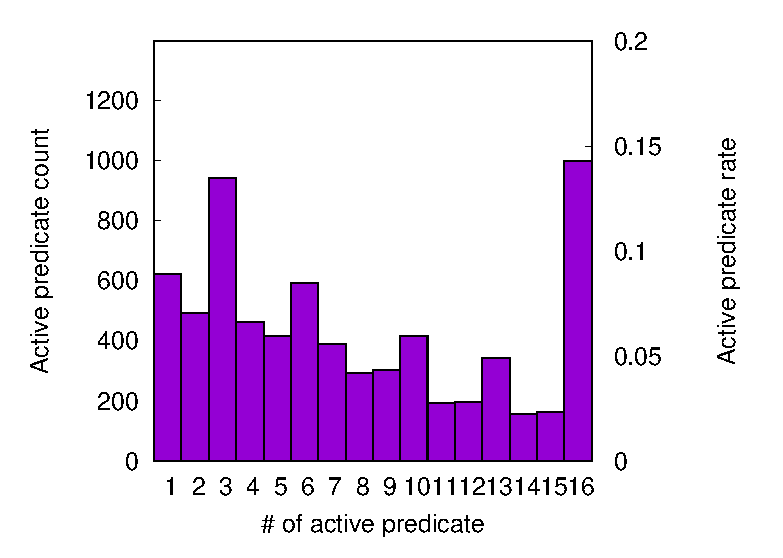
\includegraphics[width=12.0cm]{figure/lane_fill_rate.eps}
 \caption[]{SIMD幅中のアクティブなプレディケートの数及びその全体に占める割合.}
 \label{fig:lane_fill_rate}
\end{figure}

ネイバーリストのマージンを\mbox{0 \AA}から\mbox{3 \AA}まで変化させた場合の実行時間と実効性能を表\ref{tab:elapsed_time}に示す.ネイバーサーチ距離が大きくなるにしたがって,余分な計算が増えるために実行時間が長くなっている.本カーネルでは,$r^2$の計算を行った後にSIMD幅の全てのレーンがインアクティブな時に,その際の$j$粒子を相互作用計算から除外するような実装は行っていない.そのため,実行時間の増分はネイバーサーチ距離が大きくなった際のネイバーリストの長さに比例する.
示したネイバーサーチ距離の範囲では,本カーネルを使用することにより,GENESISのテーブル参照実装に比べて2.20倍から1.32倍の高速化が期待される.
 \begin{table}
  \caption{ネイバーサーチ距離とカーネル実行時間,実効性能.}
  \label{tab:elapsed_time}
  \centering
  \begin{tabular}{c c c}
   \hline \hline
   ネイバーサーチ距離(\AA) & 実行時間(ms) & 実行性能(M相互作用/s)\\ \hline
   0.0 & 0.42927 & 124.57\\
   0.5 & 0.45797 & 116.76\\
   1.0 & 0.51975 & 102.88\\
   1.5 & 0.56768 & 94.20\\
   2.0 & 0.60805 & 87.94\\
   2.5 & 0.64565 & 82.82\\
   3.0 & 0.71439 & 74.85\\
   % 0.0 & 0.480893 & 111.20 \\
   % 0.5 & 0.524780 & 101.90 \\
   % 1.0 & 0.579197 &  92.32 \\
   %  1.5 & 0.634742 &  84.24 \\
   % 2.0 & 0.689442 &  78,59 \\
   % 2.5 & 0.749041 &  71.39 \\
   % 3.0 & 0.799145 &  66.91 \\
   \hline \hline
  \end{tabular}
 \end{table}

 理想的な性能からの乖離については,$j$粒子のデータへのランダムアクセス化,相互作用パラメータの非定数化,周期境界条件の適用の順に影響が大きかった.$j$粒子のデータへのランダムアクセス化については,プリフェッチ命令が有効な場合も考えられる.

% GENESISでは,全ての粒子に対して相互作用リストを生成し,それを元に相互作用の計算を行っている.
% こちらのケースでは\ref{sec:data_align}節で述べたとおり,全ての座標データおよび相互作用のパラメータはAoS型で並んでいる.
% 本カーネルの実装では,相互作用を受ける粒子が入っているセル($i$セルと呼ぶ)から$i$セルを含むカットオフ距離内にある周囲のセル($j$セルと呼ぶ)の中にある粒子すべての粒子との距離を計算し,SIMD幅内にカットオフ距離内の粒子が1つでも存在した場合,その距離のデータを一次配列に補完しておく.そして,距離の計算が終わったら,一次配列内にある距離のデータから相互作用を計算していく.
% 2つの$i$セル内にある84の$i$粒子に対する相互作用の計算時間は\mbox{0.1845 ms}であった.
% そのため,本カーネルの計算性能は\mbox{$84 \times 723 / (0.1832 \times 10^{-3}) = 329.2$ M相互作用/sec}である.
% 作用反作用を考慮していないため,性能を半分に見ても,\ref{sec:current_situation}で示した現状のGENESISカーネル(\mbox{56.7 M相互作用/sec})の約2.90倍の性能向上である.

% ここで,$N^2$の計算からの性能低下について考える.
% 一つの$i$セルに対して,その周囲の$j$セル内にある粒子の数は少なめに見積もって5000粒子程度である.
% そして,カットオフ半径内にはおよそ720の粒子が存在する.
% そのため,$r^2$を計算するループではカットオフ半径内にある粒子数の7倍の粒子を処理していることになる.
% セルセルの演算では全体のおよそ\mbox{32.5 \%}が$r^2$の計算に使われているため,$N^2$の計算に比べて少なくとも3割弱は計算速度が低下することが予想される.
% さらに,本カーネルでは,一回の$j$ループの回転に対して,SIMD幅内の16の$i$粒子に対して一つでも相互作用の計算があれば計算が行われるため,全体のループの中でも無駄が発生している.
% 以上を考慮すると,本実装において,理想的な$N^2$の計算に対して計算速度が半分程度になってしまう程度までは妥当なラインであると結論づけた.
最後に,\ref{sec:current_situation}で示した現行GENESISの実機での測定結果と本カーネルの比較を表\ref{tab:comp}に示す.

 \begin{table}
  \caption{Nonbond\_June1と多項式近似カーネルの比較.ネイバーサーチのマージンを\mbox{1.5 \AA}と想定.}
  \label{tab:comp}
  \begin{tabular}{l||l|l}
   \hline \hline
   カーネル名 & Nonbond\_June1 & 区間多項式近似カーネル \\ \hline
   測定方法 & 実機 & 理研シミュレータ \\
   コアあたり単位時間あたりの相互作用数 & 56.7 M 相互作用/s & 87.94 M 相互作用/s \\
   1チップ48コアでの1ステップの実行時間 & 12.2 ms & 7.87 ms\\ \hline
   倍率 & $\times$1.0 & $\times$1.55 \\
   \hline \hline
  \end{tabular}
 \end{table}

 % ------No newton3 calc---------- %
% # of i-cell: 2
% # of i atoms is 80 = (16*5)
% r_c = 12.000000, r_s = 10.000000, r_m = 0.000000, b = 0.340000
% nlist[0] = 1294 (= 0 + 1294)
% nlist[1] = 1244 (= 0 + 1244)
% nlist[2] = 1641 (= 0 + 1641)
% nlist[3] = 1577 (= 0 + 1577)
% nlist[4] = 1388 (= 0 + 1388)
% # of j particles is 7144
% LIST:	   0.000512180 sec
% PRE:	   0.000001648 sec ( 0.43 %)
% POST:	   0.000000822 sec ( 0.21 %)
% r2:	   0.000134660 sec (35.05 %)
% rinv:	   0.000018369 sec ( 4.78 %)
% lj:	   0.000044516 sec (11.59 %)
% switch:	   0.000050236 sec (13.08 %)
% clmb0:	   0.000026670 sec ( 6.94 %)
% clmb1:	   0.000040136 sec (10.45 %)
% clmb2:	   0.000026152 sec ( 6.81 %)
% nwtn3:	   0.000039088 sec (10.18 %)
% other:	   0.000003785 sec ( 0.99 %)
% total time:          0.000386082 sec
% max error = 1.892090e-03, rmsf = 1.028912e-05
% ----------------- %

% ---- Newton3 calc ---- %
% # of i-cell: 2
% # of i atoms is 80 = (16*5)
% r_c = 12.000000, r_s = 10.000000, r_m = 0.000000, b = 0.340000
% NEWTON3 MODE!
% nlist[0] = 1294 (= 0 + 1294)
% nlist[1] = 1228 (= 0 + 1228)
% nlist[2] = 1609 (= 0 + 1609)
% nlist[3] = 1529 (= 0 + 1529)
% nlist[4] = 1324 (= 0 + 1324)
% # of j particles is 6984
% LIST:	   0.000503776 sec
% PRE:	   0.000001503 sec ( 0.31 %)
% POST:	   0.000001549 sec ( 0.32 %)
% r2:	   0.000128084 sec (26.75 %)
% rinv:	   0.000019010 sec ( 3.97 %)
% lj:	   0.000043459 sec ( 9.08 %)
% switch:	   0.000049158 sec (10.27 %)
% clmb0:	   0.000026428 sec ( 5.52 %)
% clmb1:	   0.000039623 sec ( 8.27 %)
% clmb2:	   0.000025630 sec ( 5.35 %)
% nwtn3:	   0.000142084 sec (29.67 %)
% other:	   0.000004265 sec ( 0.89 %)
% total time:          0.000480793 sec
% max error = 1.892090e-03, rmsf = 1.021785e-05
% ---------------------- %

\chapter{おわりに}
この文書では,分子動力学シミュレーションパッケージ「GENESIS」のLJ相互作用および静電相互作用の短距離力計算カーネルをA64FX向けに区間多項式近似を用いて最適化する手法について検討した.

現状のGENESIS Kernel\_June1はテーブルを用いて線形補間することで短距離力の計算を行っているため,性能のボトルネックはメモリおよびキャッシュへのアクセス待ちとなっている.これは,大きなテーブルを間接参照するために起こっている.
%A64FXでは近年よく用いられるようになったアクセラレータを利用したシステムに比べて改善してはいるものの,現代のシステムではバンド幅と浮動小数点演算との性能比(B/F値)は小さくなるばかりである.
%そのため,メモリアクセスがボトルネックになるようなカーネルでは,CPUの性能を十分に引き出すことは難しい.
そのため,短距離力の高速化にはメモリ上でのテーブルへの間接参照を排除し,間接アクセスを行わない高速な計算手法を開発する必要があった.

本報告書では,SIMDレジスタに収まる程度の大きさのテーブルを用いる区間多項式近似手法によるカーネルを作成し,最適化を行うことにより,実機および富士通シミュレータを用いて測定されたKernel\_June1の性能に対して,
テーブルを用いた線形近似の既存手法と同等の精度を保ちつつ1.55倍の速度向上を達成できる見込みである.

さらなる計算速度の向上の可能性としては,現状計算時間の20\%程度を占めている反作用を計算するループに関するコンパイラのバグがとれてさらなる最適化がかかること,カーネル全体のインラインアセンブラ化によるアドレス計算最適化などをすることなどが考えられる.
%今回は精度を保つために近似の精度を五次精度にしたが,筆者は4次精度でも特に問題はないと考えており,どのくらいエネルギーが保存して欲しいかどうかにあわせて近似精度を変えることも考えられる.演算が減り,使用するレジスタも減るため,後述するソフトウェアパイプライニングの段数も増加する可能性が有り,さらなる性能の向上を見込める.

\bibliographystyle{IEEEtran}
\bibliography{main}

\chapter*{付録}

\section{Skylake Xeon(実機)とA64FX(理研シミュレータ)の比較}
ARM SVEでの実装を行う前に,多項式近似カーネルの性能評価として実装した区間多項式近似(PPA)カーネルと,一般に使用されるMDシミュレーションパッケージで最速のコードのひとつであるGROMACSで用いられている方式の近距離力計算カーネルとの比較を行った.
Skylake Xeon(仕様については表\ref{tab:skylake}を参照)上で上記2つのカーネルを用いて計算を行った場合と,A64FX(理研シミュレータ)上でPPAカーネルを実行した場合の比較を図\ref{fig:comp_skylake_elapsed_time},\ref{fig:comp_skylake_performance}に示す.GROMACSに関しては,Skylake XeonとA64FXのクロック周波数の比でノーマライズしてA64FXにあわせたデータも載せている(GROMACS normalized).この比較はテスト実装で行われており,本文書で解説している実際の実装での結果とは多少異なる可能性に注意されたい.具体的には,この比較で用いたカーネルでは,相互作用を及ぼす粒子($j$粒子)がSIMD化されていること,周期境界条件を適用しない理想的な$N^2$の計算 (512粒子)での計算であることが違いとしてあげられる.また,A64FXのカーネルは実際に用いられたカーネルほどは最適化されてはいない.A64FXではGROMACS方式は実装されていないため省略する.
GROMACS方式の詳細については\url{http://manual.gromacs.org/documentation/current/doxygen/html-lib/simd__math_8h.xhtml}のpmeForceCorrectionSingleAcculacyの項を参照のこと.

  \begin{table}
   \centering
  \caption{比較に用いたSkylake Xeonの仕様.}
  \label{tab:skylake}
  \begin{tabular}{l l}
   \hline \hline
   Name & Xeon Gold 6140 \\
   Frequency & 2.30 GHz \\
   \# of cores & 18 (比較では1コアのみ使用)\\
   \hline \hline
  \end{tabular}
  \end{table}

\begin{figure}
 \centering
 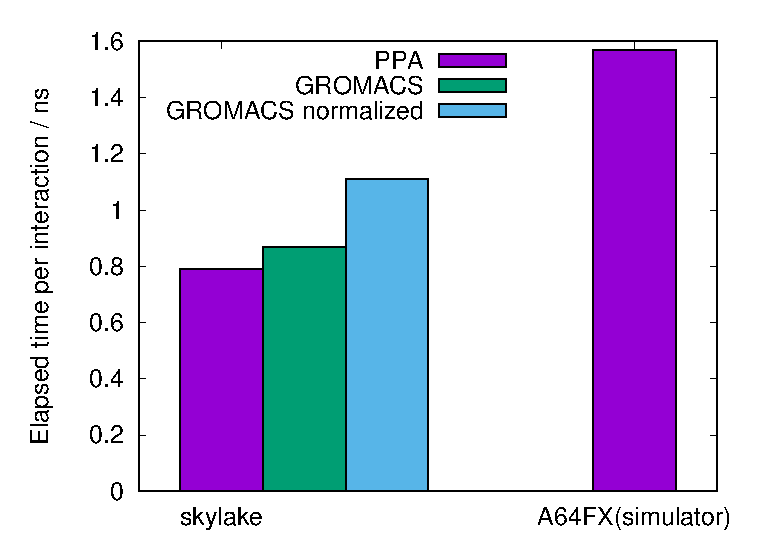
\includegraphics[width=12.0cm]{figure/comp_skylake_elapsed_time.eps}
 \caption[]{区間多項式近似(PPA)とGROMACSで採用されている方式のSkylake XeonとA64FXでの計算時間の比較.}
 \label{fig:comp_skylake_elapsed_time}
\end{figure}

\begin{figure}
 \centering
 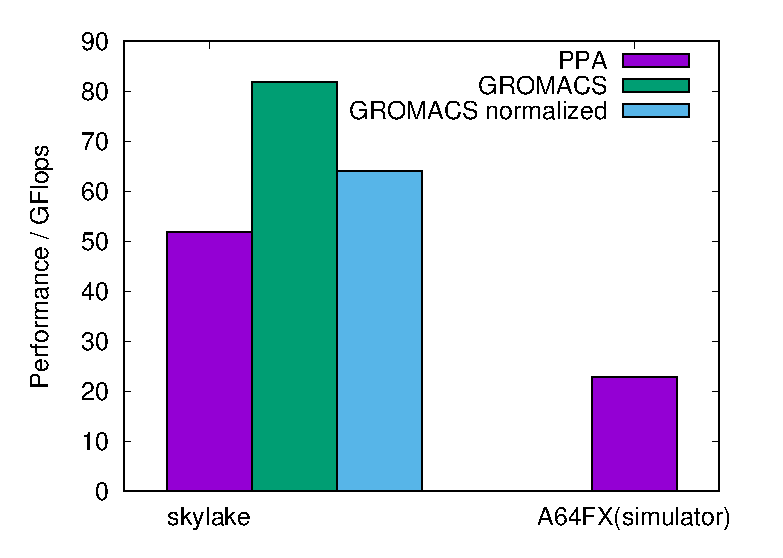
\includegraphics[width=12.0cm]{figure/comp_skylake_performance.eps}
 \caption[]{区間多項式近似(PPA)とGROMACSで採用されている方式のSkylake XeonとA64FXでの計算速度の比較.}
 \label{fig:comp_skylake_performance}
\end{figure}


\section{使用したSollyaスクリプト}
区間多項式近似の係数テーブルを作る際に用いたSollyaスクリプトをalgorithm\ref{algo:sollya}に示す.
\begin{algorithm}
 \caption{区間多項式近似カーネル用の係数を出力するSollyaスクリプト} \label{algo:sollya}
 \begin{algorithmic}
\State prec = 60;
\State f = sqrt(erfc(sqrt(x))/sqrt(x)\textasciicircum 3+2/sqrt(3.141592)*exp(-x)/sqrt(x)\textasciicircum 2);
\State for n from 0 to 2\textasciicircum 4-1 do \{
\State \ \ p = remez(f(x+((0.0078125)*2\textasciicircum n)), 5, [0;((0.0078125)*2\textasciicircum (n+1))-((0.0078125)*2\textasciicircum n)]);
\State \ \ write("\{ ");
\State \ \ for i from 0 to 5 do \{
\State \ \ \ \ write(coeff(p,i)," , ");
\State \ \ \};
\State \ \ write(" \},\textbackslash n");
\State \};
 \end{algorithmic}
\end{algorithm}

%\section{最適化オプションに依存するバグ}

 \section{最適化による演算順序の変更によるコンパイラのバグ}
% 本カーネルの相互作用・反作用の足しこみ部分には最適化の際に計算を間違えるバグが存在する.
% 該当箇所のソースコードをアルゴリズム\ref{algo:bug}に示す.
% マクロ「NO\_OPTIMIZATION」が有効化されているときは,コンパイラがループの回転数を判断することがでずSWPL等の最適化は行われない.最適化を効かせたい場合はNO\_OPTIMIZATIONを無効化した場合のように,ループの終わりを示す変数を定数にする必要がある.しかしながら,本カーネルではこのループに最適化を適用すると計算結果が変わってしまうことがわかった.このバグは,最適化オプションが-O1以上のときに起こることがわかっている.
% 原因としては,forループの終了判定をするcmp命令が吐かれないもしくは位置がおかしいことに起因している.
% そのため,本カーネルの足しこみ部分のカーネルにはSWPL等の最適化は一切行われておらず,該当部分の性能は理想的な場合に比べて著しく低い.
% 現状この部分には最適化オプションが効いていない場合,3割弱の時間が割かれているため,最適化適用による性能向上の余地は大きいと考えられる.
%このバグが発生する相互作用の足しこみおよび反作用のリダクションを行うループ内に空のアセンブラを入れることでそのループのみの最適化を抑制することができるため,このバグを回避できる.

2018年9月以前の富士通コンパイラで,本カーネルを最適化レベルO1以上でコンパイルを行うと,
SIMDの比較命令cmpXX(XXはgeやlt)が適切な順番で配置されないコンパイラのバグに起因して計算結果が変わってしまう.
該当箇所のソースコードをアルゴリズム\ref{algo:bug}に示す.
このコンパイラの最適化時のバグに関してはRedmineのFlagship2020-Aにてチケット(\#577)を切って富士通側に報告を行い,着手済みで未だチケットとしては解決にははなっていないが,
オプション「-Knosch\_pre\_ra,nosch\_post\_ra」をつけるとバグを回避できることがわかっている.もしくは,空のアセンブラを該当ループに入れるとそのループだけ最適化が効かないためバグを回避できる.
アルゴリズム\ref{algo:bug}のループの性能としては,前者の方が3割ほど良くなる.

現状,筆者が使っている理研シミュレータを実行するサーバー(plum)にインストールされている富士通コンパイラが新しくなり(2018年10月版)その場合このバグは確認されなかった.
本書で報告されているパフォーマンスや計測時間の値は旧コンパイラでバグ回避用のオプションをつけた場合で報告をしているが,
新コンパイラでオプションをつける場合とつけずに最適化を行った場合の性能差は0.4\%ほどであり,
新しいコンパイラで計測をし直しても大きな性能差は生じないと結論づけたためである.

\begin{algorithm}
 \caption{バグのあるループのコード.NO\_OPTIMIZATIONマクロを有効にすると最適化が行われず,正しく計算が行われる.バグの詳細としては,最適化によってfor文終了の比較命令とsvcmpge命令が入れ替わり,終了条件によってはfor文が早期に終了したり,長くなったりする.} \label{algo:bug}
  \begin{algorithmic}
   \State \#pragma loop norecurrence
   \State \#ifdef NO\_OPTIMIZATION
   \State for(int l=0,offset=0;\textcolor{red}{l$<$ldnl[is]};l++,offset+=16)\{
   \State \#else
   \State \textcolor{red}{const int n = ldnl[is];}
   \State for(int l=0,offset=0;\textcolor{red}{l$<$n};l++,offset+=16)\{
   \State \#endif
   \State \ \ svfloat32\_t flj = svld1\_f32(pg,f\_tmp+offset);
   \State \ \ svfloat32\_t fcl = svld1\_f32(pg,fc\_tmp+offset);
   \State \ \ flj = svadd\_f32\_z(pg,flj,fcl);
   \State \ \ svfloat32\_t dx = svld1\_f32(pg,dx\_tmp+offset);
   \State \ \ svfloat32\_t dy = svld1\_f32(pg,dy\_tmp+offset);
   \State \ \ svfloat32\_t dz = svld1\_f32(pg,dz\_tmp+offset);
   \State \ \ svfloat32\_t fx = svmul\_f32\_z(pg,flj,dx);
   \State \ \ svfloat32\_t fy = svmul\_f32\_z(pg,flj,dy);
   \State \ \ svfloat32\_t fz = svmul\_f32\_z(pg,flj,dz);
   \State \ \ fxi = svadd\_f32\_z(pg,fx,fxi);
   \State \ \ fyi = svadd\_f32\_z(pg,fy,fyi);
   \State \ \ fzi = svadd\_f32\_z(pg,fz,fzi);
   \State \ \ int j = dnl[is][l];
   \State \ \ svbool\_t excl = svcmpge\_n\_s32(pg,svdup\_n\_s32(j),i+16);
   \State \ \ f[j].x -= svaddv\_f32(excl,fx);
   \State \ \ f[j].y -= svaddv\_f32(excl,fy);
   \State \ \ f[j].z -= svaddv\_f32(excl,fz);
   \State \}
  \end{algorithmic}
\end{algorithm}


\end{document}
